\chapter*{Anexos}
\addcontentsline{toc}{chapter}{Anexos}

Los anexos reúnen el material de respaldo del experimento: el registro visual de las capturas, la configuración del puerto plano, los perfiles de calibración, la referencia geométrica del riel, la estructura de los repositorios de código y datos, la tabla maestra de resultados, las fichas de las réplicas y las fotografías del montaje y de los instrumentos. Los archivos completos están publicados con los datos del experimento (Anexo~\ref{anx:repositorio}); aquí se muestran sus campos principales para facilitar la lectura y la trazabilidad.

\chapter{Registro visual de capturas}
\label{anx:capturas}

La Figura~\ref{fig:A-1} reúne en una sola vista las capturas del experimento. Cada etiqueta indica la réplica, la repetición y la distancia nominal de la réplica al vidrio en milímetros; por ejemplo, \texttt{R1-REP1-50.jpg}. La vista permite comprobar la organización del conjunto y la correspondencia de cada captura con su posición. Las 72 imágenes originales están publicadas en el repositorio de datos (Anexo~\ref{anx:repositorio}).

\begin{figure}[H]
\centering
\caption[Vista conjunta de las capturas y sus identificadores]{Vista conjunta de las capturas y sus identificadores.}
\label{fig:A-1}
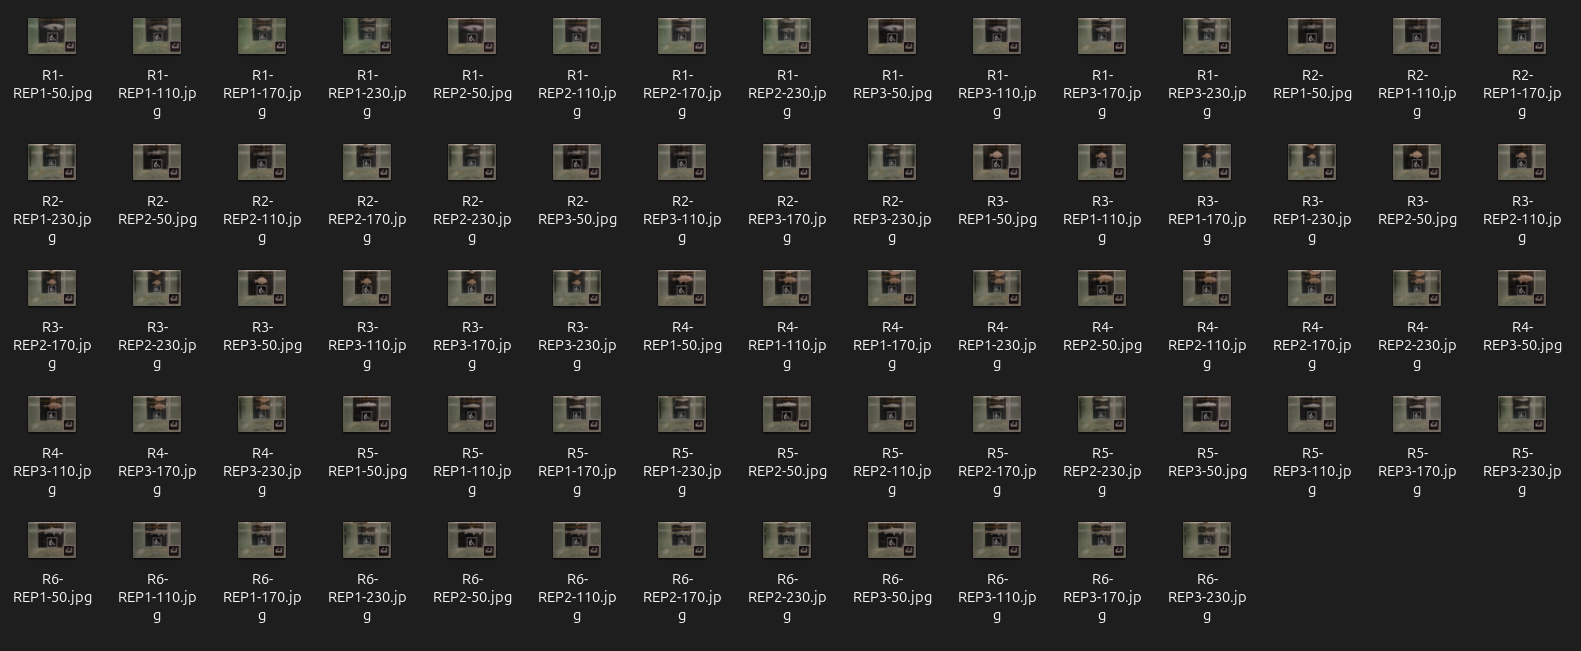
\includegraphics[width=\textwidth]{figA_1_capturas.png}
\fignota{Elaboración propia.}
\end{figure}

\chapter{Configuración del puerto plano}
\label{anx:flatport}

La Figura~\ref{fig:B-1} reproduce la configuración del modelo de puerto plano, resumida en la Tabla~\ref{tab:puerto}: unidades en milímetros, normal de cámara $(0, 0, 1)$, distancia de la interfaz de 230~mm, vidrio de 4~mm de espesor e índices de refracción de 1,000 para el aire, 1,500 para el vidrio y 1,333 para el agua. El archivo deja constancia de que la distancia de la lente se midió desde su frente, como aproximación, y de que el agua estaba a 22~\si{\celsius}, con salinidad 0 y presión 0~dbar.

\begin{figure}[H]
\centering
\caption[Parámetros visibles de la configuración del puerto plano]{Parámetros visibles de la configuración del puerto plano.}
\label{fig:B-1}
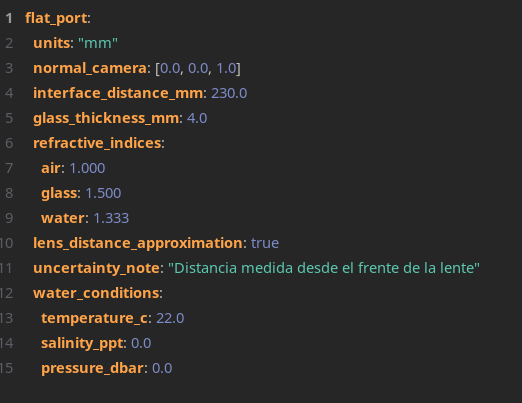
\includegraphics[width=0.6\textwidth]{figB_1_flatport.png}
\fignota{Captura de pantalla de Fishmeter, aplicación desarrollada en este trabajo.}
\end{figure}

\chapter{Parámetros de calibración de cámara}
\label{anx:calibraciones}

Los archivos \texttt{calibration\_B.yaml} y \texttt{calibration\_C\_air.yaml} guardan los perfiles de calibración de las rutas B y C. Los dos usan el modelo de cámara de OpenCV, una resolución de $4096 \times 3072$ píxeles y un tablero de $4 \times 4$ esquinas interiores con cuadros de 20~mm. La Tabla~\ref{tab:calibraciones} presenta sus indicadores de calidad. Los listados que siguen reproducen la cabecera y el resumen de cada archivo; los informes de cada vista quedan en los YAML completos, publicados con los datos (Anexo~\ref{anx:repositorio}).

\begin{lstlisting}[caption={Cabecera y resumen del perfil B.},label={lst:calB}]
schema: fish_morphometry.b_calibration.v1
profile_id: B-effective
profile_hash: eb245104cb46caded48e9e9f827dda11db985c7b22ec5cb63a27572da14caf4e
calibration_context_hash: 1e3531dcf0d9ff8d00b322b41d2dd074b41cb822a1324cd5545635303ca81ba6
model: OPENCV
camera_matrix:
- [4502.32284117, 0.0, 2027.2736574393155]
- [0.0, 4504.395746404586, 1549.0026630316365]
- [0.0, 0.0, 1.0]
distortion_coefficients:
- 0.4454686711747631
- -3.4668133596510753
- -0.008336348094703296
- 0.004790603340447537
- 8.25240238252019
resolution: [4096, 3072]
calibration_rail_position_mm: 0.0
created_at_utc: '2026-10-12T04:07:10.722788+00:00'
versions:
  opencv: 5.0.0
  fish_morphometry: 0.1.0
source: opencv_calibrateCamera
board:
  inner_corners: [4, 4]
  square_size_mm: 20.0
rms_px: 0.4353568098178903
views:
  received: 35
  accepted: 35
  rejected: 0
\end{lstlisting}

\begin{lstlisting}[caption={Cabecera y resumen del perfil C en aire.},label={lst:calC}]
schema: fish_morphometry.air_calibration.v1
profile_id: C-air
profile_hash: fb98aea6af6ba57d663f5884b4034bfff3413c62cc376bef82256a7c1f412a55
calibration_context_hash: 623631f83c66f4b1615fd73e2f4db719880ccaa11c117bc705674d1a0df96ef8
model: OPENCV
camera_matrix:
- [3313.72125140631, 0.0, 2028.1975106019397]
- [0.0, 3313.6744263215105, 1530.5739559303083]
- [0.0, 0.0, 1.0]
distortion_coefficients:
- 0.18564347583186028
- -0.829350911254369
- -0.0011635185172718578
- -0.0015902497923188043
- 1.0012733784385703
resolution: [4096, 3072]
board:
  inner_corners: [4, 4]
  square_size_mm: 20.0
  units: mm
rms_px: 0.3745461951579489
created_at_utc: '2026-10-12T04:12:38.034127+00:00'
versions:
  opencv: 5.0.0
  fish_morphometry: 0.1.0
source: opencv_calibrateCamera_air
views:
  received: 36
  accepted: 36
  rejected: 0
\end{lstlisting}

\chapter{Referencia geométrica del riel para B}
\label{anx:riel}

El archivo \texttt{rail\_reference\_B.yaml} documenta el plano de referencia de B, obtenido a partir de dos posiciones del riel, 0 y 180~mm, con un error de reproyección de 0,270~px (umbral de 1,0~px). El ajuste informa un residuo lineal de $1{,}62 \times 10^{-13}$~mm, que es el residuo numérico de una recta por dos puntos y no representa la incertidumbre física; una dispersión de la normal de $0{,}337^{\circ}$ (umbral de $1{,}0^{\circ}$); y un error relativo de escala de 0,813~\% (umbral de 5~\%). El archivo registra además dos supuestos: los planos de las réplicas son paralelos al tablero, y el riel no es necesariamente perpendicular a él. La Tabla~\ref{tab:riel} resume los valores principales.

\begin{lstlisting}[caption={Cabecera y plano de referencia del riel para B.},label={lst:riel}]
plane_point_camera_mm:
- -34.117491789288806
- -28.291160700295567
- 365.1469994117171
plane_normal_camera:
- -0.03972877728543376
- -0.042783728187314775
- 0.9982941334385363
z_ref_mm: 0.0
rail_direction_camera:
- 0.02095849070805215
- -0.04478647483729878
- 0.998776708448334
\end{lstlisting}

\chapter{Repositorio de código y datos}
\label{anx:repositorio}

El trabajo está publicado en dos repositorios. El código de Fishmeter está en \url{\RepoURL}, etiqueta \texttt{\RepoTag}, que corresponde al commit\par\noindent{\footnotesize\texttt{\RepoCommit}}\par
\noindent Los datos del experimento y los scripts que regeneran las tablas y figuras del Capítulo~\ref{cap:resultados} están en el repositorio de este documento, \url{\DatosURL}, etiqueta \texttt{\DatosTag}, que corresponde al commit\par\noindent{\footnotesize\texttt{\DatosCommit}}\par\noindent La estructura de ambos es la siguiente:

\begin{lstlisting}
FishmeterTPF/                     codigo (etiqueta v1.0-tesis)
  src/fish_morphometry/           aplicacion Fishmeter (calibracion, geometria,
                                  metodos A, A', B y C, interfaz, validacion)
  tests/                          pruebas unitarias e integracion (pytest)
  docs/                           guia de uso y notas de desarrollo
  README.md                       instalacion y ejecucion

ProyectoTPF/                      datos y analisis
  datos/imagenes/                 72 imagenes JPG originales
  datos/calibraciones/            perfiles B y C, puerto plano y riel (YAML)
  datos/referencias/replicas.csv  tres lecturas de calibre por medida
  datos/resultados_json/          un JSON por imagen y metodo (puntos y parametros)
  datos/derivados/                L(z), intervalos y sensibilidad de C
  datos/SHA256SUMS                huellas de todos los archivos de datos
  datos/README.md                 contenido y convenciones de los datos
  anexos/csv-maestro-re-run.csv   tabla maestra (288 registros)
  analysis/reproducir_capitulo4.py  Tablas 4.3 a 4.6, pruebas de signos,
                                  Bland-Altman y Figuras 4.5 y 4.6
  analysis/make_figures.py        Figuras 4.1 a 4.4 y 4.7
  analysis/tabla_maestra.py       tabla del Anexo F
  analysis/re_run_b.py            recalculo de B con la lectura del riel
\end{lstlisting}

Para reproducir el Capítulo~\ref{cap:resultados} se debe instalar Fishmeter en la versión indicada y ejecutar, desde la raíz de ProyectoTPF, los tres primeros scripts de \texttt{analysis/} en el orden del listado. El primero recalcula C desde los puntos marcados con el perfil \texttt{C-air} y la configuración del puerto plano; los otros dos leen la tabla maestra, los resultados del primero y, para la Figura~\ref{fig:4-captura}, la imagen original. El cuarto, \texttt{re\_run\_b.py}, documenta cómo se obtuvieron los valores de B de la tabla maestra: toma los JSON de B del cálculo preliminar y repite el cálculo con la posición expresada en el marco del riel (Anexo~\ref{anx:riel}), sin cambiar los puntos marcados ni las calibraciones. Su salida ya está incluida en la tabla maestra, por lo que no es necesario ejecutarlo para reproducir el capítulo.

\chapter{Tabla maestra de resultados}
\label{anx:maestra}

La Tabla~\ref{tab:maestra} reproduce, para cada una de las 72 imágenes, las referencias de calibre y las estimaciones de LT y PC de los cuatro métodos; el error con signo de cada estimación es su diferencia con la referencia. Los guiones marcan los cuatro registros sin valor, en los que no se detectó el ArUco (Sección~\ref{sec:conjunto}). La tabla se generó con \texttt{analysis/tabla\_maestra.py} a partir del CSV maestro, que guarda además los puntos marcados (con $\mathbf{p}_1$ y $\mathbf{p}_2$ invertidos respecto de la definición de la Sección~\ref{sec:medidas}), los parámetros de cada ruta y sus advertencias. Su huella SHA-256 figura a continuación de la tabla.

% Generado por analysis/tabla_maestra.py; no editar a mano.
% CSV: csv-maestro-re-run.csv, SHA-256 f5e8c1091ceb06ec406dffc0d1a02f5b65f9147fdf5a582671e33e65abf8235c
\newcommand{\MaestraSHA}{f5e8c1091ceb06ec406dffc0d1a02f5b65f9147fdf5a582671e33e65abf8235c}
\begin{footnotesize}
\setlength{\tabcolsep}{4pt}
\begin{longtable}{@{}lrrrrrrrrrr@{}}
\caption{Tabla maestra: referencias de calibre y estimaciones por imagen y método.}
\label{tab:maestra}\\
\toprule
 & \multicolumn{5}{c}{Longitud total (mm)} & \multicolumn{5}{c}{Profundidad corporal (mm)} \\
\cmidrule(lr){2-6}\cmidrule(l){7-11}
Imagen & Ref. & A & \Aprime & B & C & Ref. & A & \Aprime & B & C \\
\midrule
\endfirsthead
\toprule
 & \multicolumn{5}{c}{Longitud total (mm)} & \multicolumn{5}{c}{Profundidad corporal (mm)} \\
\cmidrule(lr){2-6}\cmidrule(l){7-11}
Imagen & Ref. & A & \Aprime & B & C & Ref. & A & \Aprime & B & C \\
\midrule
\endhead
\bottomrule
\endfoot
\texttt{R1-REP1-50} & 158,7 & 143,0 & 161,8 & 162,7 & 164,1 & 45,0 & 41,0 & 45,6 & 45,9 & 46,8 \\
\texttt{R1-REP2-50} & 158,7 & 143,2 & 164,7 & 156,9 & 158,1 & 45,0 & 40,8 & 46,7 & 44,2 & 45,0 \\
\texttt{R1-REP3-50} & 158,7 & 142,7 & 163,8 & 156,4 & 157,6 & 45,0 & 41,3 & 47,5 & 44,7 & 45,5 \\
\texttt{R1-REP1-110} & 158,7 & 123,0 & 163,3 & 163,6 & 164,7 & 45,0 & 34,7 & 45,7 & 45,6 & 46,3 \\
\texttt{R1-REP2-110} & 158,7 & 123,2 & 162,4 & 157,3 & 158,4 & 45,0 & 35,2 & 46,1 & 44,5 & 45,2 \\
\texttt{R1-REP3-110} & 158,7 & 123,4 & 161,8 & 157,5 & 158,6 & 45,0 & 35,0 & 45,3 & 44,3 & 45,0 \\
\texttt{R1-REP1-170} & 158,7 & 106,9 & 164,1 & 162,2 & 163,3 & 45,0 & 30,2 & 45,9 & 45,2 & 45,9 \\
\texttt{R1-REP2-170} & 158,7 & 108,1 & 162,6 & 157,7 & 158,8 & 45,0 & 30,8 & 46,4 & 44,6 & 45,3 \\
\texttt{R1-REP3-170} & 158,7 & 108,5 & 163,5 & 158,4 & 159,5 & 45,0 & 30,7 & 46,1 & 44,4 & 45,1 \\
\texttt{R1-REP1-230} & 158,7 & 94,5 & 163,5 & 161,3 & 162,5 & 45,0 & 26,5 & 45,6 & 44,8 & 45,5 \\
\texttt{R1-REP2-230} & 158,7 & 95,9 & 161,9 & 157,6 & 158,9 & 45,0 & 27,4 & 46,1 & 44,8 & 45,5 \\
\texttt{R1-REP3-230} & 158,7 & 96,0 & 162,5 & 157,9 & 159,1 & 45,0 & 27,3 & 45,9 & 44,5 & 45,2 \\
\texttt{R2-REP1-50} & 134,3 & 119,1 & 136,5 & 131,2 & 132,1 & 27,3 & 24,6 & 28,2 & 26,5 & 27,0 \\
\texttt{R2-REP2-50} & 134,3 & 120,4 & 135,0 & 132,6 & 133,5 & 27,3 & 25,5 & 28,4 & 27,5 & 28,0 \\
\texttt{R2-REP3-50} & 134,3 & 120,6 & 136,5 & 132,9 & 133,8 & 27,3 & 25,1 & 28,4 & 27,0 & 27,5 \\
\texttt{R2-REP1-110} & 134,3 & 103,6 & 135,1 & 133,2 & 134,1 & 27,3 & 21,6 & 28,0 & 27,2 & 27,6 \\
\texttt{R2-REP2-110} & 134,3 & 104,6 & 136,7 & 134,3 & 135,2 & 27,3 & 21,5 & 28,1 & 27,0 & 27,5 \\
\texttt{R2-REP3-110} & 134,3 & 103,7 & 135,1 & 133,3 & 134,2 & 27,3 & 21,7 & 28,1 & 27,4 & 27,8 \\
\texttt{R2-REP1-170} & 134,3 & 90,6 & 137,0 & 133,1 & 134,1 & 27,3 & 18,7 & 28,3 & 26,9 & 27,4 \\
\texttt{R2-REP2-170} & 134,3 & --- & --- & 133,5 & 134,5 & 27,3 & --- & --- & 27,1 & 27,6 \\
\texttt{R2-REP3-170} & 134,3 & 91,0 & 135,5 & 133,8 & 134,8 & 27,3 & 19,1 & 28,3 & 27,6 & 28,0 \\
\texttt{R2-REP1-230} & 134,3 & 80,7 & 135,8 & 133,4 & 134,5 & 27,3 & 16,9 & 28,4 & 27,5 & 27,9 \\
\texttt{R2-REP2-230} & 134,3 & 80,6 & 136,0 & 133,2 & 134,3 & 27,3 & 16,6 & 28,2 & 26,9 & 27,4 \\
\texttt{R2-REP3-230} & 134,3 & 80,9 & 135,0 & 133,6 & 134,8 & 27,3 & 16,9 & 28,1 & 27,5 & 27,9 \\
\texttt{R3-REP1-50} & 91,7 & 82,6 & 93,8 & 91,2 & 91,8 & 40,3 & 37,0 & 42,5 & 40,2 & 40,9 \\
\texttt{R3-REP2-50} & 91,7 & --- & --- & 91,4 & 92,0 & 40,3 & --- & --- & 40,1 & 40,8 \\
\texttt{R3-REP3-50} & 91,7 & 83,0 & 93,8 & 91,6 & 92,2 & 40,3 & 36,9 & 41,9 & 40,1 & 40,7 \\
\texttt{R3-REP1-110} & 91,7 & 71,4 & 94,2 & 91,9 & 92,6 & 40,3 & 31,5 & 41,5 & 40,0 & 40,6 \\
\texttt{R3-REP2-110} & 91,7 & 71,4 & 93,2 & 91,9 & 92,6 & 40,3 & 32,1 & 41,4 & 40,7 & 41,4 \\
\texttt{R3-REP3-110} & 91,7 & 71,2 & 93,2 & 91,8 & 92,5 & 40,3 & 31,9 & 41,6 & 40,5 & 41,2 \\
\texttt{R3-REP1-170} & 91,7 & 62,1 & 93,1 & 91,5 & 92,3 & 40,3 & 28,0 & 41,8 & 40,7 & 41,3 \\
\texttt{R3-REP2-170} & 91,7 & 62,4 & 93,9 & 91,9 & 92,6 & 40,3 & 28,0 & 42,2 & 40,7 & 41,3 \\
\texttt{R3-REP3-170} & 91,7 & 62,3 & 93,6 & 91,8 & 92,6 & 40,3 & 28,1 & 42,0 & 40,8 & 41,5 \\
\texttt{R3-REP1-230} & 91,7 & 55,4 & 93,7 & 91,7 & 92,6 & 40,3 & 24,5 & 41,6 & 40,1 & 40,7 \\
\texttt{R3-REP2-230} & 91,7 & 55,9 & 93,3 & 92,4 & 93,3 & 40,3 & 24,7 & 41,1 & 40,3 & 40,9 \\
\texttt{R3-REP3-230} & 91,7 & 55,4 & 93,3 & 91,8 & 92,7 & 40,3 & 24,7 & 41,3 & 40,4 & 41,1 \\
\texttt{R4-REP1-50} & 142,7 & 130,5 & 149,3 & 143,5 & 144,5 & 42,7 & 39,0 & 44,6 & 42,0 & 42,8 \\
\texttt{R4-REP2-50} & 142,7 & 132,5 & 150,1 & 145,9 & 146,9 & 42,7 & 39,7 & 45,2 & 42,7 & 43,6 \\
\texttt{R4-REP3-50} & 142,7 & 133,0 & 148,9 & 146,1 & 147,1 & 42,7 & 39,6 & 44,2 & 42,6 & 43,4 \\
\texttt{R4-REP1-110} & 142,7 & 113,7 & 148,7 & 145,9 & 146,8 & 42,7 & 33,5 & 43,6 & 42,2 & 42,9 \\
\texttt{R4-REP2-110} & 142,7 & 114,1 & 148,7 & 146,1 & 147,0 & 42,7 & 33,6 & 43,6 & 42,2 & 42,9 \\
\texttt{R4-REP3-110} & 142,7 & 114,0 & 148,8 & 146,3 & 147,2 & 42,7 & 34,2 & 44,3 & 43,1 & 43,9 \\
\texttt{R4-REP1-170} & 142,7 & 99,4 & 148,5 & 145,7 & 146,7 & 42,7 & 29,6 & 44,5 & 42,7 & 43,3 \\
\texttt{R4-REP2-170} & 142,7 & 99,3 & 149,0 & 145,7 & 146,7 & 42,7 & 29,3 & 43,9 & 42,2 & 42,9 \\
\texttt{R4-REP3-170} & 142,7 & 99,5 & 149,1 & 145,7 & 146,7 & 42,7 & 29,2 & 43,7 & 42,0 & 42,7 \\
\texttt{R4-REP1-230} & 142,7 & 87,4 & 147,6 & 144,3 & 145,4 & 42,7 & 25,9 & 43,3 & 42,1 & 42,7 \\
\texttt{R4-REP2-230} & 142,7 & 88,4 & 148,3 & 145,8 & 146,9 & 42,7 & 26,4 & 44,0 & 42,8 & 43,5 \\
\texttt{R4-REP3-230} & 142,7 & 87,3 & 147,4 & 144,1 & 145,2 & 42,7 & 25,9 & 43,6 & 42,1 & 42,8 \\
\texttt{R5-REP1-50} & 137,3 & 123,8 & 139,1 & 136,3 & 137,2 & 25,7 & 22,4 & 25,0 & 24,1 & 24,6 \\
\texttt{R5-REP2-50} & 137,3 & 124,2 & 139,6 & 136,5 & 137,4 & 25,7 & 22,8 & 25,6 & 24,5 & 25,0 \\
\texttt{R5-REP3-50} & 137,3 & 124,5 & 140,3 & 136,8 & 137,8 & 25,7 & 23,0 & 26,0 & 24,7 & 25,2 \\
\texttt{R5-REP1-110} & 137,3 & 106,8 & 139,7 & 137,1 & 138,1 & 25,7 & 19,8 & 26,2 & 24,9 & 25,4 \\
\texttt{R5-REP2-110} & 137,3 & 106,9 & 141,3 & 137,3 & 138,3 & 25,7 & 19,6 & 25,9 & 24,5 & 25,0 \\
\texttt{R5-REP3-110} & 137,3 & 107,2 & 140,5 & 137,3 & 138,3 & 25,7 & 20,0 & 26,1 & 25,1 & 25,6 \\
\texttt{R5-REP1-170} & 137,3 & 93,3 & 139,6 & 136,9 & 137,9 & 25,7 & 16,9 & 25,3 & 24,3 & 24,8 \\
\texttt{R5-REP2-170} & 137,3 & 93,3 & 139,9 & 136,7 & 137,7 & 25,7 & 17,1 & 25,6 & 24,6 & 25,0 \\
\texttt{R5-REP3-170} & 137,3 & 93,6 & 140,7 & 137,1 & 138,1 & 25,7 & 16,7 & 25,0 & 24,0 & 24,4 \\
\texttt{R5-REP1-230} & 137,3 & 82,7 & 140,8 & 136,7 & 137,9 & 25,7 & 14,8 & 25,4 & 24,0 & 24,5 \\
\texttt{R5-REP2-230} & 137,3 & 82,0 & 138,9 & 135,4 & 136,6 & 25,7 & 15,1 & 25,3 & 24,4 & 24,8 \\
\texttt{R5-REP3-230} & 137,3 & 82,9 & 139,4 & 136,7 & 137,9 & 25,7 & 15,1 & 25,2 & 24,4 & 24,8 \\
\texttt{R6-REP1-50} & 209,7 & 189,8 & 213,2 & 208,7 & 210,0 & 35,3 & 33,6 & 37,8 & 36,2 & 36,9 \\
\texttt{R6-REP2-50} & 209,7 & 189,7 & 212,2 & 208,0 & 209,3 & 35,3 & 32,8 & 36,3 & 35,3 & 36,0 \\
\texttt{R6-REP3-50} & 209,7 & 189,6 & 212,6 & 208,1 & 209,4 & 35,3 & 32,5 & 36,2 & 35,0 & 35,7 \\
\texttt{R6-REP1-110} & 209,7 & 162,3 & 212,7 & 207,7 & 208,7 & 35,3 & 28,7 & 37,7 & 36,2 & 36,8 \\
\texttt{R6-REP2-110} & 209,7 & 163,0 & 212,3 & 208,5 & 209,6 & 35,3 & 27,6 & 35,9 & 34,7 & 35,3 \\
\texttt{R6-REP3-110} & 209,7 & 163,4 & 212,4 & 208,8 & 209,8 & 35,3 & 28,1 & 36,6 & 35,3 & 35,9 \\
\texttt{R6-REP1-170} & 209,7 & 142,8 & 211,2 & 208,8 & 209,9 & 35,3 & 25,3 & 36,9 & 36,5 & 37,1 \\
\texttt{R6-REP2-170} & 209,7 & 142,9 & 213,9 & 208,8 & 209,9 & 35,3 & 24,5 & 36,7 & 35,3 & 35,8 \\
\texttt{R6-REP3-170} & 209,7 & 143,2 & 213,4 & 209,0 & 210,1 & 35,3 & 23,9 & 35,1 & 34,4 & 35,0 \\
\texttt{R6-REP1-230} & 209,7 & 127,0 & 216,0 & 208,8 & 210,1 & 35,3 & 21,3 & 36,4 & 34,7 & 35,2 \\
\texttt{R6-REP2-230} & 209,7 & 126,4 & 214,2 & 208,3 & 209,6 & 35,3 & 21,1 & 35,3 & 34,4 & 35,0 \\
\texttt{R6-REP3-230} & 209,7 & 126,2 & 211,5 & 207,4 & 208,7 & 35,3 & 21,4 & 35,5 & 34,7 & 35,2 \\
\end{longtable}
\end{footnotesize}


\noindent{\footnotesize SHA-256 del CSV maestro:\\ \texttt{\MaestraSHA}}

\chapter{Fichas de las réplicas}
\label{anx:fichas}

Las seis réplicas están impresas en PLA. La Figura~\ref{fig:G-1} las muestra juntas, cada una con su identificador, y la Tabla~\ref{tab:lecturas-calibre} reproduce las tres lecturas de calibre de cada medida, registradas al milímetro, con su media y su desviación estándar muestral; las medias son las referencias de la Tabla~\ref{tab:replicas}.

\begin{figure}[H]
\centering
\caption[Réplicas utilizadas en el experimento con su identificador]{Las seis réplicas impresas en PLA, con el identificador (R1--R6) que se usa en todo el documento.}
\label{fig:G-1}
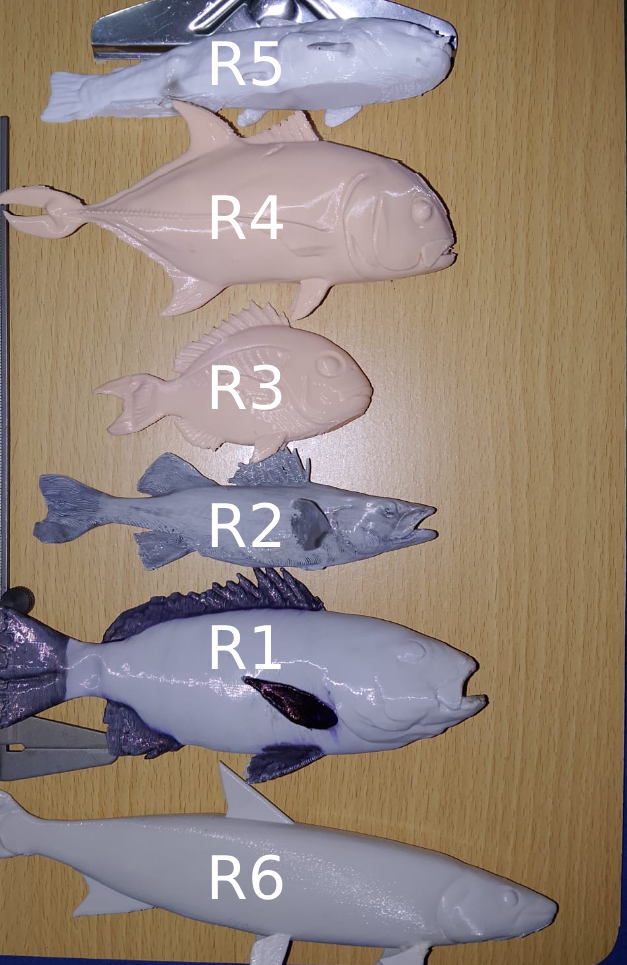
\includegraphics[width=0.55\textwidth]{fig3_1_replicas_tags.jpg}
\fignota{Elaboración propia.}
\end{figure}

\begin{table}[H]
\centering\footnotesize
\caption{Lecturas de calibre de las réplicas (mm).}
\label{tab:lecturas-calibre}
\begin{tabular}{@{}lccccc@{\hspace{1.2em}}ccccc@{}}
\toprule
 & \multicolumn{5}{c}{Longitud total (LT)} & \multicolumn{5}{c}{Profundidad corporal (PC)} \\
\cmidrule(lr){2-6}\cmidrule(l){7-11}
Réplica & 1 & 2 & 3 & Media & Desv. & 1 & 2 & 3 & Media & Desv. \\
\midrule
R1 & 160 & 157 & 159 & 158,7 & 1,5 & 45 & 45 & 45 & 45,0 & 0,0 \\
R2 & 131 & 136 & 136 & 134,3 & 2,9 & 28 & 27 & 27 & 27,3 & 0,6 \\
R3 & 91  & 92  & 92  & 91,7  & 0,6 & 41 & 40 & 40 & 40,3 & 0,6 \\
R4 & 141 & 146 & 141 & 142,7 & 2,9 & 43 & 42 & 43 & 42,7 & 0,6 \\
R5 & 137 & 138 & 137 & 137,3 & 0,6 & 25 & 26 & 26 & 25,7 & 0,6 \\
R6 & 210 & 209 & 210 & 209,7 & 0,6 & 35 & 36 & 35 & 35,3 & 0,6 \\
\bottomrule
\end{tabular}

\smallskip
\begin{minipage}{0.9\textwidth}\footnotesize
\emph{Nota.} Las lecturas de PC de R1 y R2 se anotaron originalmente con un cero de más (450 por 45~mm; 280/270/270 por 28/27/27~mm) y se corrigieron antes del análisis; la corrección está registrada en \texttt{datos/referencias/replicas.csv} y en la tabla maestra.
\end{minipage}
\end{table}

\chapter{Montaje e instrumentos}
\label{anx:montaje}

La Figura~\ref{fig:H-1} muestra la pecera de vidrio en la que se hizo el ensayo, con agua y el soporte de PLA en su interior; sus dimensiones y la disposición del montaje están en la Sección~\ref{sec:montaje} y en la Figura~\ref{fig:3-esquema}. La Figura~\ref{fig:H-2} reúne los instrumentos con los que se midió y se armó el montaje: las reglas y la escuadra con las que se midió la distancia cámara--vidrio y se comprobó la perpendicularidad de la cámara, el calibre analógico con el que se tomaron las medidas de referencia, el damero de calibración, los dos marcadores ArUco, el soporte del teléfono y los útiles con los que se cortaron y fijaron las piezas.

\begin{figure}[H]
\centering
\caption[Pecera utilizada en el experimento]{Pecera de vidrio utilizada en el experimento, con agua y el soporte de PLA en su interior.}
\label{fig:H-1}
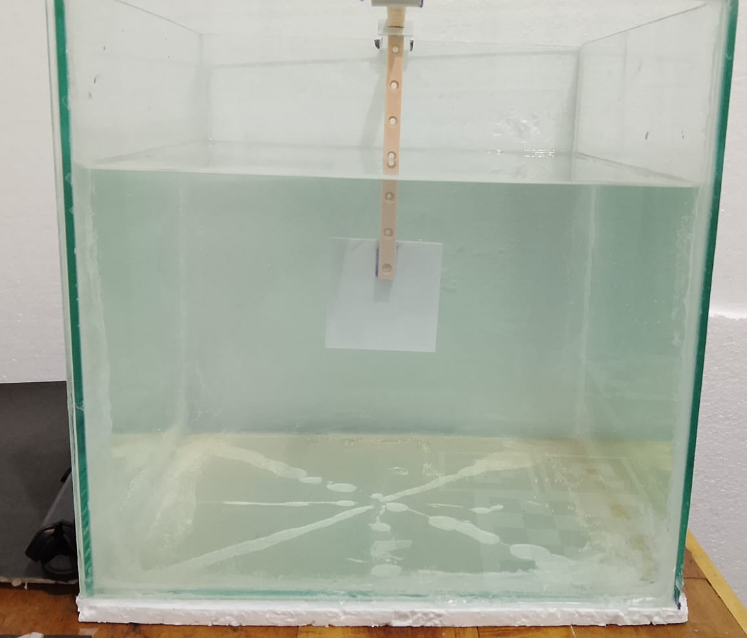
\includegraphics[width=0.48\textwidth]{estanque.png}
\fignota{Elaboración propia.}
\end{figure}

\begin{figure}[H]
\centering
\caption[Instrumentos de medición y de manipulación]{Instrumentos de medición y de manipulación: reglas, escuadra, calibre, damero de calibración, marcadores ArUco, soporte del teléfono, cinta doble faz y herramientas de corte y sujeción.}
\label{fig:H-2}
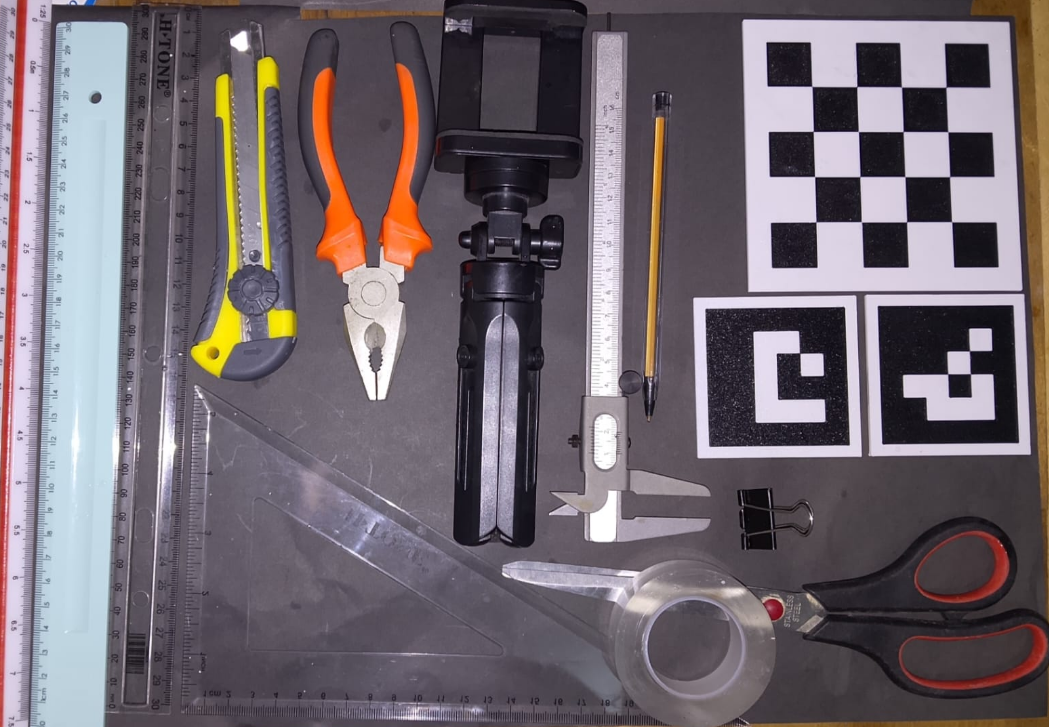
\includegraphics[width=0.65\textwidth]{tools-measure-manipulate.png}
\fignota{Elaboración propia.}
\end{figure}


% ---------------------------------------------------------------------------
% Registro de cambios: comentado para la entrega. Para mostrarlo de nuevo,
% seleccionar las líneas siguientes y quitar el comentario (Ctrl+/).
% ---------------------------------------------------------------------------
% \chapter{Registro de cambios de esta versión}
% \label{anx:cambios}
%
% Esta versión del documento incorpora las observaciones de dos revisiones independientes realizadas el 13 de octubre de 2026 sobre la versión anterior del libro (77 páginas). El registro siguiente permite justificar cada cambio y lo que no se incorporó, conforme al artículo 17 del Reglamento de Proyecto Final. La numeración A-$n$ y B-$n$ remite a las correcciones de cada revisión.
%
% \begin{footnotesize}
% \begin{longtable}{@{}p{1.6cm}p{2.0cm}p{6.0cm}p{5.0cm}@{}}
% \caption{Registro de cambios respecto de la versión anterior.}
% \label{tab:registro-cambios}\\
% \toprule
% Ref. & Ubicación anterior & Cambio realizado & Motivo \\
% \midrule
% \endfirsthead
% \toprule
% Ref. & Ubicación anterior & Cambio realizado & Motivo \\
% \midrule
% \endhead
% \bottomrule
% \endfoot
% \endlastfoot
% A-1, B-26 & Cap.~1 y 2 & Los verbos en futuro que describían acciones realizadas pasaron a pretérito; las definiciones a presente; lo no realizado se declara como pendiente. & El documento informa una investigación concluida. \\
% A-2, A-6, B-01 & Título, 1.5, 1.6, 4.6 & Se agregó la Sección~\ref{sec:intervalo} con la estimación geométrica del ancho de $\IL$ y su verificación contra el error de A; la corrida numérica de $L(z)$ sobre las 72 capturas, su ancho y su cobertura se incorporaron a la Tabla~\ref{tab:intervalo} y a la Figura~\ref{fig:4-Lz}. & El título y la pregunta principal prometían el intervalo y ninguna sección lo trataba. Se mantiene el título. \\
% A-3, B-04/05 & 1.8, 4.4 & H1 y H2 reescritas con criterios coincidentes con lo calculado; nueva Sección~\ref{sec:contraste} con tabla de veredictos; H2 declarada no sostenida e interpretada. & No existía contraste de hipótesis; los datos refutaban H2 sin decirlo. \\
% A-4, B-03 & 1.6, Cap.~4 & Secciones~\ref{sec:repetibilidad} y~\ref{sec:sensibilidad} creadas con sus tablas; matriz de cumplimiento en la Tabla~\ref{tab:cumplimiento}. & Objetivos 2, 5 y 6 sin resultado. \\
% A-5, B-27 & pp.~8, 11, 19, 27, 30, 54, 62 & Eliminadas las frases de proceso («D7 del informe», «2-antecedente.tex», «carpeta anexo/», fila «pendiente de verificación»). & Texto dirigido al autor, no al lector. \\
% A-7, B-12 & pp.~42--48 & Reemplazado «requiere comprobación física independiente / resultados exploratorios» por la descripción del estado interno del software y la validación contra calibre; distinción entre comprobación con patrón y validación externa. & La comparación contra calibre es la validación física. \\
% A-8, B-07 & pp.~42--49 & Las cinco menciones a la advertencia de unidad de PC de R1 y R2 se concentraron en un recuadro pendiente de la Sección~\ref{sec:conjunto}, que se retiró al corregir los valores en la Tabla~\ref{tab:replicas}. & Es una tarea de medición, no una limitación. \\
% B-08 & 4.3 & La inferencia se hizo con la réplica como unidad (prueba de signos, $n = 6$, $p = 0{,}031$); los conteos 24/24 pasan a descriptivos. & Las 24 combinaciones son medidas repetidas de seis réplicas. \\
% B-09, B-10 & 3.7, 4.1 & Se aclara que las métricas describen la estimación promedio por condición y que el pareamiento no es idéntico en dos combinaciones; el recálculo con la intersección de las 70 imágenes comunes no cambió ningún valor en más de 0,01. & Rigor del diseño pareado. \\
% A-9, B-23 & 3.3, Anexo E & Hash completo del commit y etiqueta prevista; Anexo~\ref{anx:repositorio} con el árbol del repositorio; publicación de datos pendiente. & Reproducibilidad. \\
% A-10, B-15 & Cap.~3 & Tabla~\ref{tab:replicas} de réplicas y referencias (media y desviación de tres lecturas; origen del modelo pendiente); lado físico de los ArUco verificado con calibre (cuadrado negro de 60~mm; 70~mm con el margen blanco). & El lector debe conocer contra qué se comparó. \\
% A-11 & Cap.~4 & Figuras~\ref{fig:4-1}, \ref{fig:4-2} y~\ref{fig:4-3} generadas por script desde las tablas. & El capítulo no tenía figuras. \\
% A-12, B-24 & Resumen & Resumen y abstract reescritos con hallazgos y conclusión (menos de 350 palabras), sin tareas pendientes. & Anexo I del reglamento. \\
% A-13, B-18 & Cap.~1 & 1.2 ampliado; Sección~\ref{sec:conclusiones}; nueva 1.9.1 de delimitación; Tabla~\ref{tab:trazabilidad}. & Estructura del Anexo I y trazabilidad. \\
% A-14, B-22 & Cap.~3 & 3.1 renombrada con tipo, enfoque, población y muestra; Tabla~\ref{tab:operacionalizacion}; Tablas~\ref{tab:puerto} y~\ref{tab:riel} subidas desde los anexos. & Marco metodológico del Anexo I. \\
% A-15 & 4.5 & Párrafo sobre B reescrito: sesgo constante como error de escala, con la razón de focales 1,36. & Convertir una contradicción en un hallazgo interpretado. \\
% A-16, B-43 & 5.5 & Párrafo con el aporte a la Ingeniería Informática; Tabla~\ref{tab:regla} y Figura~\ref{fig:5-1}. & Explicitar el aporte de la carrera. \\
% A-17 & 5.4 & Trabajos futuros separados en verificaciones inmediatas y líneas de continuación. & Evitar leer el trabajo futuro como lista de incumplimientos. \\
% A-18, B-28 & 2.7, Tabla 2.1 & Párrafo y filas de MorphoCal, Yin y Zhou con los datos verificados de las fuentes primarias. & Una fila «pendiente de verificación» es inadmisible en la versión final. \\
% A-19, B-16/17 & 2.5, 3.4, 3.5 & Definición operacional de $\mathbf{p}_2$ y de LT; fórmula implementada de la escala (ecuación~\ref{eq:escala-impl}); homografía de \Aprime{} y plano de B formulados; nombres de funciones retirados del cuerpo. & Coherencia texto--código y rigor. \\
% A-20, B-45 & 3.2 & Efecto de medir $d$ desde el frente de la lente acotado analíticamente y calculado numéricamente (Tabla~\ref{tab:sensibilidad}). & Pregunta previsible de la mesa. \\
% A-21 & 2.2 & Orden «aire--vidrio--agua» unificado en todo el documento. & Concordancia. \\
% A-22 & 4.2 & Fórmulas definidas una sola vez en la Sección~\ref{sec:evaluacion}. & Concisión. \\
% A-23 & 1.1 & Introducción reducida a tres párrafos; el estado del arte queda en 2.7. & Concisión. \\
% A-24/25/26/27, B-38/39/41 & Preliminares & Orden según el Anexo I; numeración romana única; tildes; «Tutora: Ing. Evelyn Giménez»; «para optar al título de Ingeniero en Informática»; \texttt{hidelinks}. & Formato. \\
% A-28 & Acrónimos & Lista reducida a las siglas usadas. & Rúbrica, ítem 5. \\
% A-29 a A-33, B-36, B-42 & varias & Erratas («La Los», «no se se», «çorrección»), cita parentética, cita narrativa de CalibMar, «Petrellis (2021) combinó», concordancia de $\mathbf{n}_\pi$, lados de $\Pi_1$ y $\Pi_2$, «Listado». & Corrección y uniformidad. \\
% A-34, A-36, B-30/33 & Referencias & Hartley y Zisserman, Brown, Hecht, Shortis, Bland y Altman y Lin agregados; Genovese, Huai, Waleed, Rojtberg y Markvorsen retirados; Weng, Tseng, Correia, Torres, Marrable, Qiao, Steeds, Petrellis y Saleh corregidos. Pendientes: DOI de Seegräber (2025) y páginas de Torres (2018). & APA 7 y pertinencia. \\
% A-35 & Figuras & Leyenda completa de la Figura~\ref{fig:2-3}; fuente en todas las figuras. & Formato. \\
% A-37 & 2.7 & Se indicó el número de trabajos seleccionados (catorce, Tabla~\ref{tab:antecedentes}) y de resultados adicionales examinados (alrededor de veinte). & Trazabilidad de la búsqueda. \\
% A-38 & 3.3 & Versiones de Python, OpenCV, NumPy y PyYAML. & Reproducibilidad. \\
% A-39 & 3.8, 5.2 & Limitaciones metodológicas y de resultados separadas. & Concisión. \\
% §6 de A & 3.9 & Nueva Sección~\ref{sec:etica} de cuestiones éticas y uso de herramientas. & Anexo I; transparencia. \\
% B-13, B-14 & 3.2, Anexo D & Tabla~\ref{tab:posiciones} de correspondencia de posiciones (lecturas del riel completadas; desplazamiento al plano de simetría pendiente); residuo del riel aclarado como numérico. & Dos orígenes sin correspondencia; número vacío presentado como evidencia. \\
% B-20, B-21, B-29 & 2.3, 2.2.7, 4.8 & Atribución causal precisada (coplanaridad + homografía; modelo completo + profundidad); CalibMar como antecedente, calibraciones con OpenCV y trazado propio. & Honestidad del instrumento y de la atribución. \\
% Concordancia & Cap.~3 y 4; Anexos & Comprobación de las cifras contra el CSV maestro y los datos de $L(z)$: identificadores de los ArUco corregidos en la Figura~\ref{fig:3-esquema}; C frente a B en PC, 23 de 24 combinaciones; redondeos de la Tabla~\ref{tab:posiciones-mae}; MAE por captura en la Tabla~\ref{tab:agregados}; lado de los ArUco medido con calibre; lecturas de calibre en la Tabla~\ref{tab:lecturas-calibre}; redacción de la sensibilidad a $\mu_w$; Tablas~\ref{tab:sensibilidad} y~\ref{tab:intervalo} verificadas sin diferencias. Se detectó que B se ejecutó con el plano desplazado 50~mm; su recálculo queda pendiente. & Concordancia entre texto y datos. \\
% Recálculo de B & Cap.~3, 4 y 5; Resumen; Abstract & B se volvió a ejecutar con la lectura del riel ($z - 50$~mm) en lugar de la distancia al vidrio; se rehicieron las Tablas~\ref{tab:agregados} y~\ref{tab:posiciones-mae}, la comparación pareada, H1 (ahora sostenida frente a A y \Aprime{} y no frente a B) y H2, la discusión, el resumen, el abstract y las conclusiones; se agregaron la Figura~\ref{fig:4-errores}, la Figura~\ref{fig:4-captura} y la Tabla~\ref{tab:maestra}. & Error de entrada detectado en la comprobación de concordancia. \\
% No incorporado & Título & No se cambió el título propuesto por la revisión B. & El título está registrado y la Sección~\ref{sec:intervalo} responde la pregunta que enuncia; el cambio quedaba como contingencia si la corrida de $L(z)$ no se realizaba; la corrida se realizó. \\
% No incorporado & Resumen & No se incluyeron en el resumen las tareas pendientes (comprobación instrumental), como proponía la revisión B. & El resumen informa hallazgos; las salvedades están en las Secciones~\ref{sec:conjunto} y~\ref{sec:limitaciones-metod}. \\
% \end{longtable}
% \end{footnotesize}
%
% Los recuadros «PENDIENTE» distribuidos en el cuerpo del documento (\thependcount{} en total) señalan los puntos que requieren datos o cálculos no disponibles al preparar esta versión. Deben resolverse y eliminarse antes de la entrega definitiva.
